In our project we are also focused on developing a visualisation tool
for \textsc{PureCircuit} instances. 
In our introduction we referred to three main objectives. As of time of writing
we are close to the completion of the first one. We will provide a table of
objectives that have been achieved, as well as the remaining requirements needed
to complete the first milestone in \ref{tab:soft:rem-unrem-issues-stage1}. Lastly, we provide a figure
of our current visualisation in \ref{fig:soft:current-phases}

\begin{table}[h!]
    \centering
    \begin{tabularx}{0.9\textwidth}{|Y|Y|}
            \hline
            \textbf{Accomplished} & \textbf{Finished} \\
            \hhline{|==|}
            Ability to add and move nodes                                  & Add values to value nodes                                                                                   \\ \hline
            Toggle between value nodes and gate nodes                                  & Specify the type of gate to add                                                                             \\ \hline
            Add edges. Ensure that edges can only be added between heterogeneous nodes & Add indicators as to how many edges are excess/remaining for the gate to be valid                           \\ \hline  
            Move whole graph                                                           & Inclusion of a status bar as to whether the current assignment is correct, wrong or syntactically incorrect \\  \hline
            Create panel to show current state as well as some indicator and guides    &   \\ \hline
    \end{tabularx}
    \caption{Finished and remaining issues}\label{tab:soft:rem-unrem-issues-stage1}
\end{table}

%%Add image visualisation
\begin{figure}[h!]
    \centering
    \subfloat[Add nodes]{
        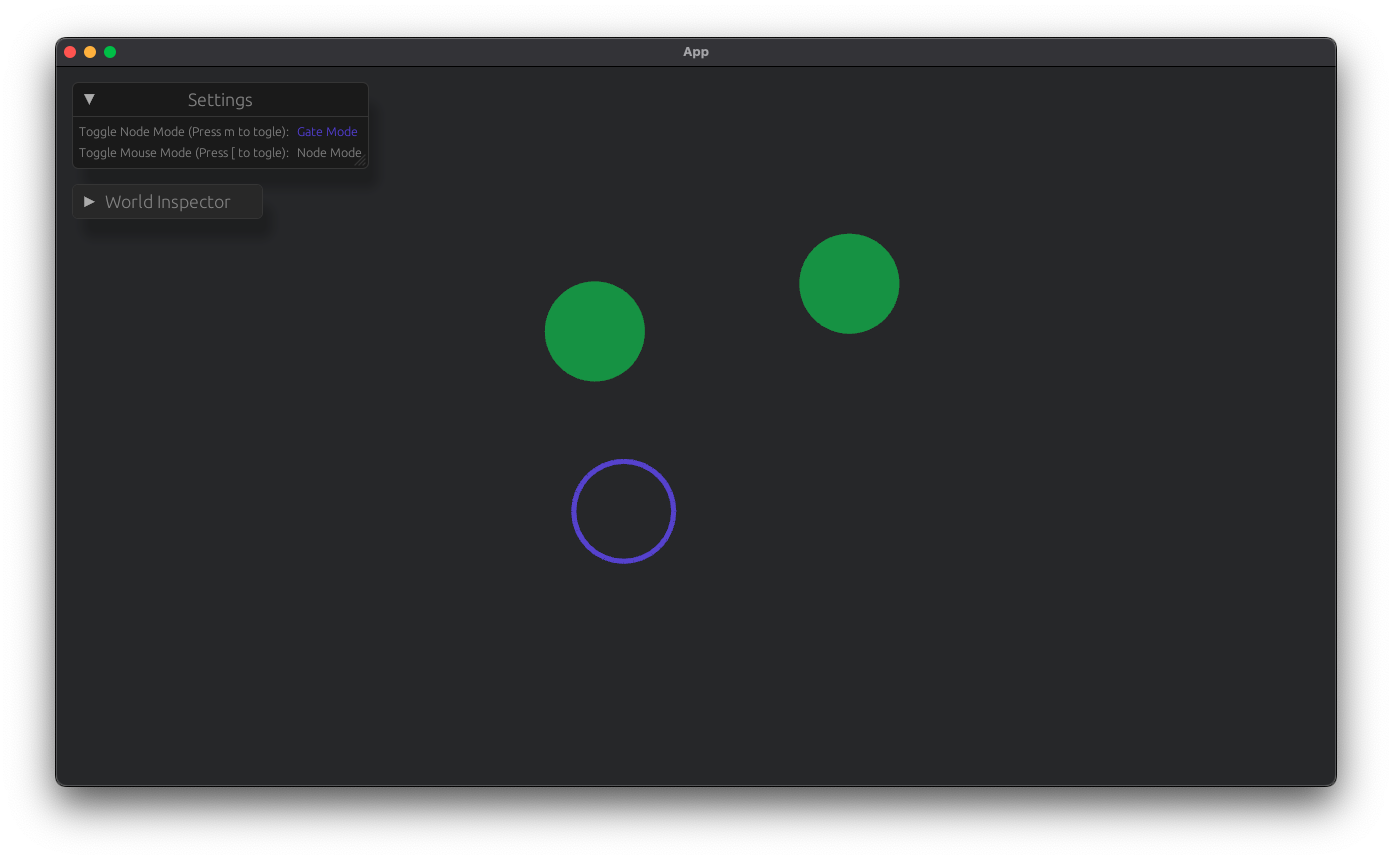
\includegraphics[width=0.3\linewidth]{assets/soft-phase-1-add-node.png}
        \label{fig:soft-phase-1:add-node}
    }
    \subfloat[Add edges]{
        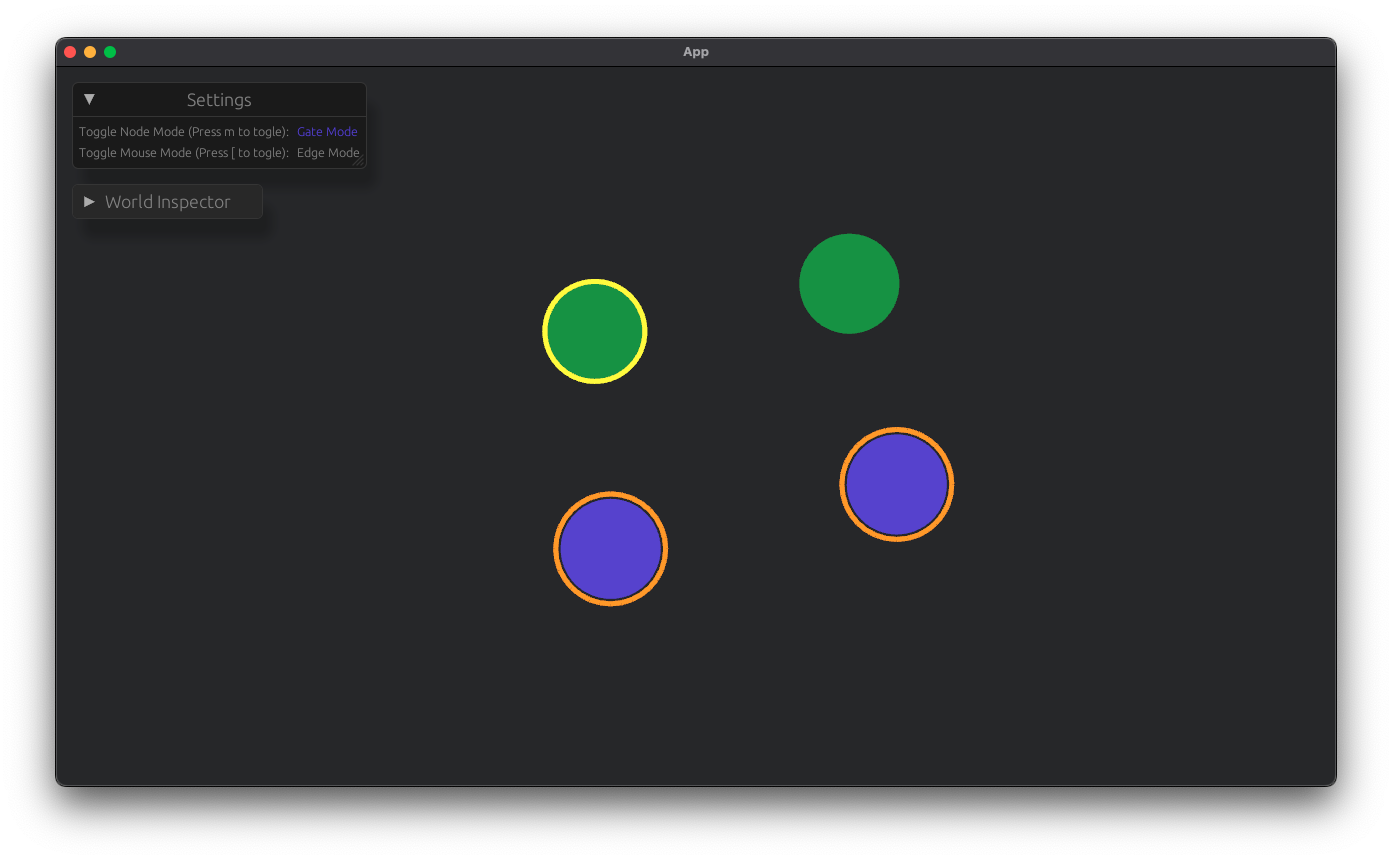
\includegraphics[width=0.3\linewidth]{assets/soft-phase-1-add-edge.png}
        \label{fig:soft-phase-1:add-edge}
    }
    \subfloat[Final state]{
        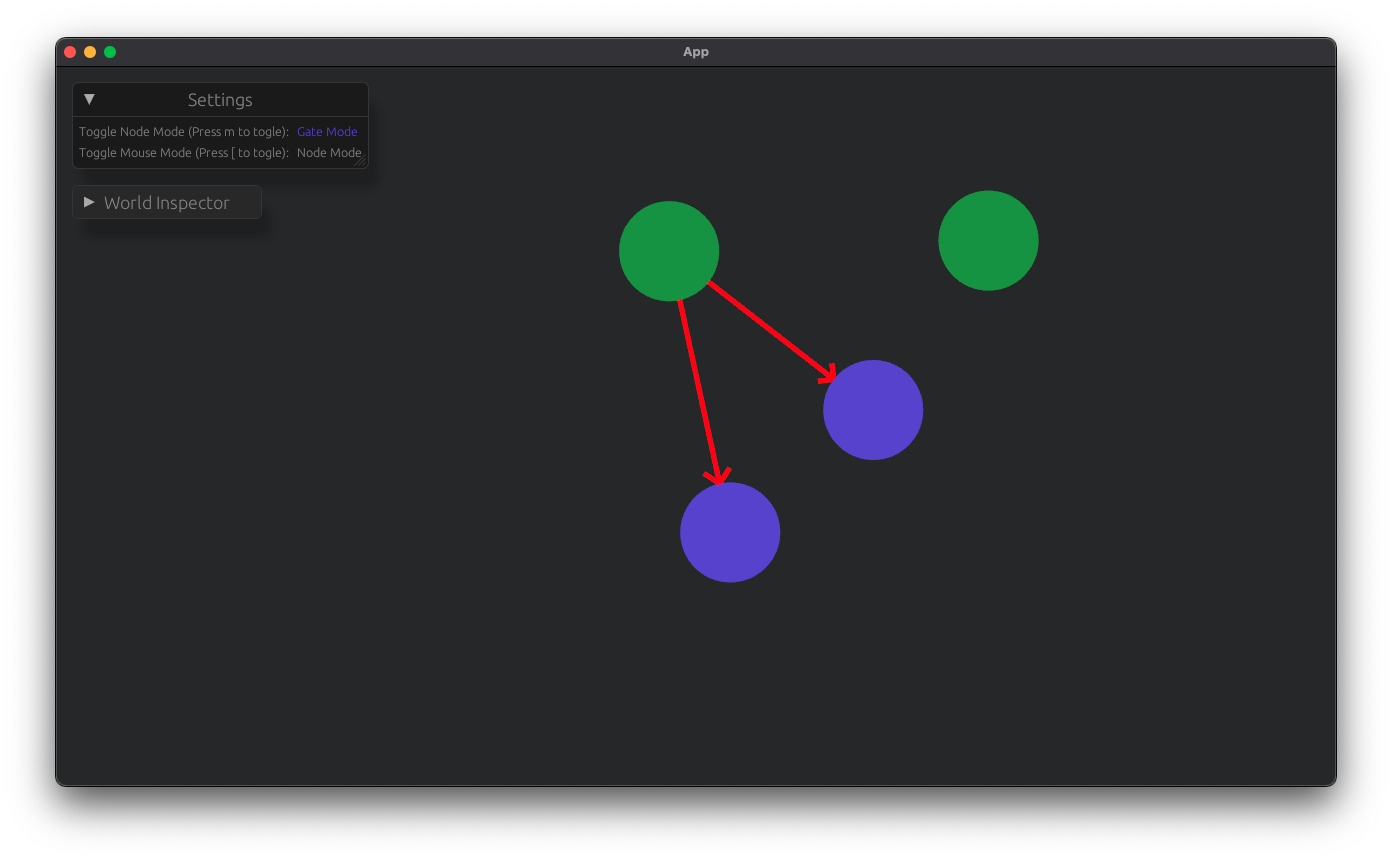
\includegraphics[width=0.3\linewidth]{assets/ soft-phase-1-final-state.png}
        \label{fig:soft-phase-1:final-state}
    }
    \caption{Screenshots of different states of the visualisation tool}
    \label{fig:soft:current-phases}
\end{figure}





